% !TEX TS-program = pdflatex
% !TEX encoding = UTF-8 Unicode

% This is a simple template for a LaTeX document using the "article" class.
% See "book", "report", "letter" for other types of document.

\documentclass[11pt]{article} % use larger type; default would be 10pt

\usepackage[utf8]{inputenc} % set input encoding (not needed with XeLaTeX)

%%% Examples of Article customizations
% These packages are optional, depending whether you want the features they provide.
% See the LaTeX Companion or other references for full information.

%%% PAGE DIMENSIONS
\usepackage{geometry} % to change the page dimensions
\geometry{a4paper} % or letterpaper (US) or a5paper or....
% \geometry{margin=2in} % for example, change the margins to 2 inches all round
% \geometry{landscape} % set up the page for landscape
%   read geometry.pdf for detailed page layout information

\usepackage{graphicx} % support the \includegraphics command and options

% \usepackage[parfill]{parskip} % Activate to begin paragraphs with an empty line rather than an indent

%%% PACKAGES
\usepackage{float}
\usepackage{booktabs} % for much better looking tables
\usepackage{array} % for better arrays (eg matrices) in maths
\usepackage{paralist} % very flexible & customisable lists (eg. enumerate/itemize, etc.)
\usepackage{verbatim} % adds environment for commenting out blocks of text & for better verbatim
\usepackage{subfig} % make it possible to include more than one captioned figure/table in a single float
% These packages are all incorporated in the memoir class to one degree or another...

%%% HEADERS & FOOTERS
\usepackage{fancyhdr} % This should be set AFTER setting up the page geometry
\pagestyle{fancy} % options: empty , plain , fancy
\renewcommand{\headrulewidth}{0pt} % customise the layout...
\lhead{}\chead{}\rhead{}
\lfoot{}\cfoot{\thepage}\rfoot{}

%%% SECTION TITLE APPEARANCE
\usepackage{sectsty}
\allsectionsfont{\sffamily\mdseries\upshape} % (See the fntguide.pdf for font help)
% (This matches ConTeXt defaults)

%%% ToC (table of contents) APPEARANCE
\usepackage[nottoc,notlof,notlot]{tocbibind} % Put the bibliography in the ToC
\usepackage[titles,subfigure]{tocloft} % Alter the style of the Table of Contents
\renewcommand{\cftsecfont}{\rmfamily\mdseries\upshape}
\renewcommand{\cftsecpagefont}{\rmfamily\mdseries\upshape} % No bold!

%%% Definitions
\def\mbh{{\rm M_{\rm BH}}}
\def\macc{{\rm M_{\rm acc}}}
\def\mdisc{{\rm M_{\rm disc}}}
\def\vturb{ v_{\rm turb} }
\def\rcirc{r_{\rm rirc}}
\def\racc{r_{\rm acc}}
\def\rdisc{r_{\rm disc}}
\def\tilt{\theta_{\rm tilt}}
\def\pc{\rm ~pc}
\def\kpc{\rm ~kpc}
\def\km{\rm ~km}
\def\kms{\rm ~km/s}
\def\msun{\rm ~M_\odot}
\def\msunyr{\rm ~M_\odot/ yr}

%%% END Article customizations

%%% The "real" document content comes below...

\title{Counter-Rotating Flows - checklist}
\author{Juan Manuel Carmona Loaiza - jcarmona@sissa.it}
%\date{Trieste, Italy. April 4, 2013} % Activate to display a given date or no date (if empty),
         % otherwise the current date is printed 

\begin{document}
\maketitle
\begin{figure}[H]
\includegraphics[width=\textwidth]{./Discs}
\end{figure}

\vspace{1cm}

The main parameters of our simulations when letting fall a single gaseous shell into the SMBH are its initial angular momentum, $l_0$; the level of turbulence, $v_{\rm turb}$; and the mass of the central black hole $\mbh$ (newly introduced for this study). In the following list I propose a series of simulations to be done in order to better understand the implications that counter-rotating flows proposed in Carmona-Loaiza et al. (2014, 2015) have for SMBH accretion.

\section{Sanity check: reproducing analytical estimates.}

As sanity check, we need to perform test simulations (low resolution?) in which we vary the parameters $l_0$ and $\mbh$ and see how the accreted mass, $\macc$, and circularization radius, $r_{\rm circ}$ compare to analytical estimates. We would be testing the following quantities: $\rcirc(l_0,\mbh)$ and $\macc(l_0,\mbh)$ by performing the following simulations:\\


$\bullet$ Fix $v_0 = 0.3 \, (l_0 = 0.018)$ and let $\mbh = 10^{\{6,7,8,9\}}$.

$\bullet$ Fix $\mbh = 10^8$ and let $v_0 = \{0.1, 0.2, 0.3, 0.5, 0.7\}$\\

Number of simulations: $8$.\\

\noindent We should reproduce the plots shown in Figure \ref{fig: rcirc}.\\

\begin{figure}
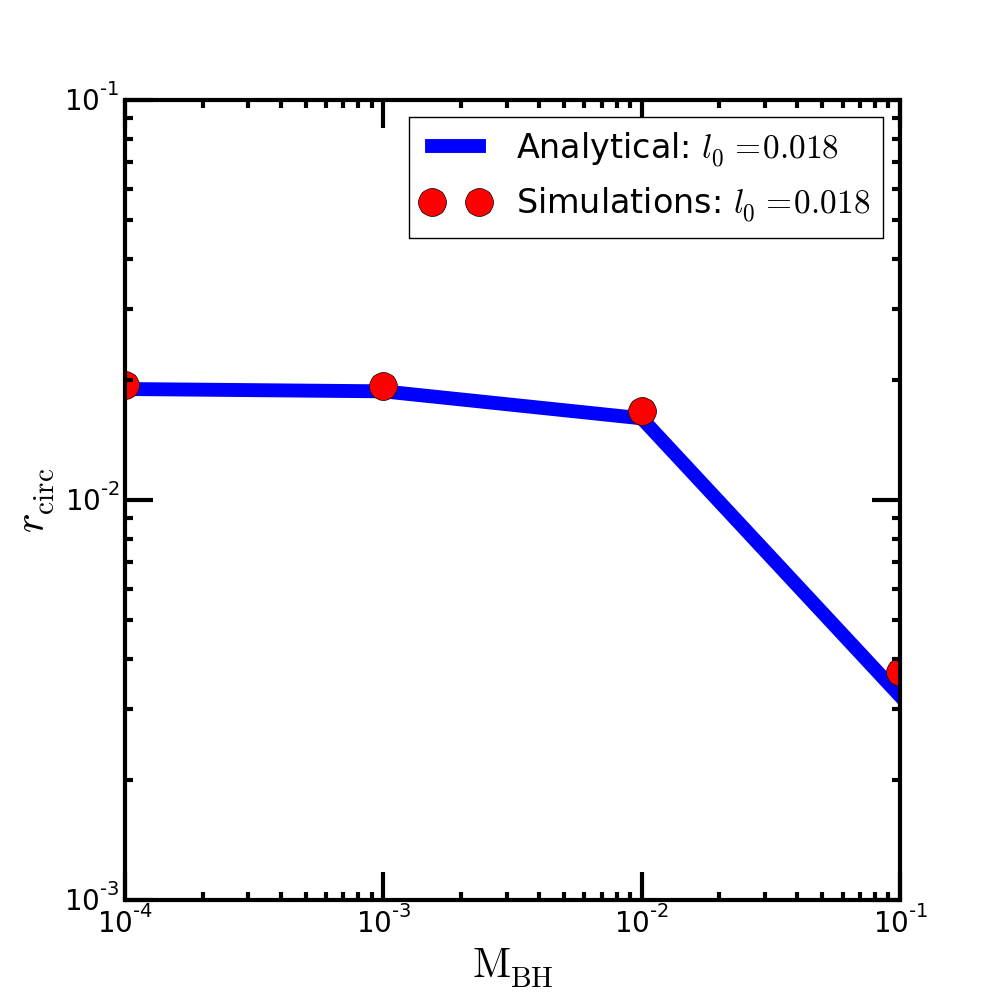
\includegraphics[width=0.49\textwidth]{./rcirc_mbh}
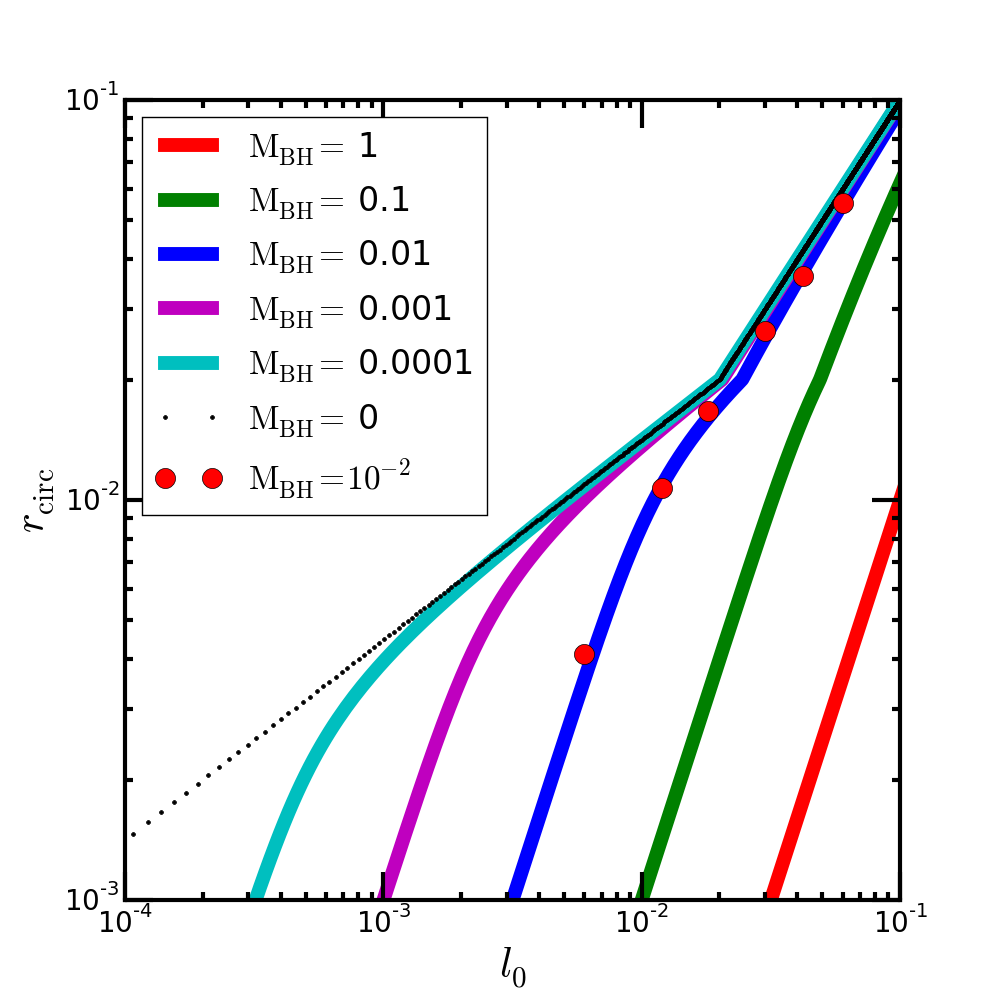
\includegraphics[width=0.49\textwidth]{./rcirc_l0}
\caption{In the left panel we fix $l_{0}$, the initial mean angular momentum of the shell, and observe how is the rircularization radius $\rcirc$ changes when varying $\mbh$. In the right panel we do the opposite: keep fixed $\mbh$ and see how the circularization radius behaves with changing $l_0$. This analytical computations should be reproduce by our simulations. Otherwise we should understand and estimate the source of error.}
\label{fig: rcirc}

\end{figure}

\noindent Additionally, we should make two more simulations with different accretion radius: \\

$\bullet$ $\racc << \tilde{r}$ (or even with no $\racc$) and measure $M(r<\tilde{r})$.

$\bullet$ $\racc = \tilde{r}$ and measure $\macc$.\\

Number of simulations: $2$-$4$.\\

\noindent Ideally we should expect $M(r<\tilde{r}) = \macc$, however, due to numerical viscosity this won't be the case. This couple of simulations should tell us how much we are overestimating the accretion of mass with respect to the accretion radius and the circularization radius (if $\tilde{r}  = \rcirc$).\\



\section{How turbulence affects accretion and shape of the disc.}

Additionally, it would be desirable to have a measure of how turbulence affects the density profile of the disc that is created after the infall of the shell has finished, together with the accreted mass. For this, the following simulations are proposed (Basically reproducing the results by Hobbs et al. 2011):\\

$\bullet$ Fix $v_0 = 0.3$, $M_bh = 10^8$, and let $\vturb = {0.1, 0.2, 0.3, 0.5, 0.7, 1.0}$\\
	
Number of simulations: $6$.\\

\noindent As a sanity check, I would propose an extra group of simulations to measure how well the effects of turbulence are being captured by our resolution and which is the minimum resolution to reach convergence, both in shape and in accreted mass:\\

$\bullet $Fix $v_0 = 0.3$, $\mbh = 10^8$, and $\vturb = \{ v_{\alpha}, v_{\beta} \}$, 

$\bullet$ Repeat for $N_{\rm particles} =$ 100k?, 200k, 500k, 1M?\\

Number of simulations: 2-8,\\

\noindent with $v_{\alpha,\beta}$ representing the turbulence velocities for which the resulting disc was thinner/wider (or the accretion was greater/smaller).\\

\section{Misaligned inflows}

At this stage I would create a brand new disc with my own desired density profile, $\Sigma(\mdisc,\rdisc)$, to put it inside a new gaseous shell. Only at this point is that the interaction between the inner disc and the shell will be studied, treating misalignment, $\tilt$, and the properties of the disc, $\rdisc$ and $\mdisc$, as new parameters. As from my previous studies we already know something about how the accretion  grows when misaligned inflows interact, and from the other simulations we're planning we should gather knowledge of the behaviour of $\macc$ with respect to $\vturb$ and $\mbh$, we can focus this time on the new parameters in flows for which $L_{\rm z, disc} = - L_{\rm z, shell}$. I would propose the following simulations, which would tell us something new and interesting to extract some conclusions:\\

$\bullet$ Fix $\Sigma$ and $\tilt$. Test three different values of $\vturb$.

$\bullet$ Fix $\Sigma$ and $\vturb$. Test three different values of $\tilt$.

$\bullet$ Fix $\vturb$, $\tilt$ and $\mdisc$. Test three different values of $\rdisc$.

$\bullet$ Fix $\vturb$, $\tilt$ and $\rdisc$. Test three different values of $\mdisc$.\\

\noindent Number of simulations: 9\\

\noindent [Grand total number of simulations to be done: 27 - 35]

\end{document}

%Bibliography:
%Accretion Power in Astrophysics (Juhan Frank, Andrew King, Derek Raine)
%An article written by John Miller, Annalisa Celotti and Sciama about observational evidence of BH
%1939 famous article by Oppenheimer and Snider
%How massive single stars end their life (Heger et al. 2003)
%Stephan Rosswog - Introduction to High Energy Astrophysics
%Malcolm Longair - High Energy Astrophysics (Vol IV?)
%Jogee 2004 - The Fueling and Evolution of AGN: Internal and External Triggers
%Hopkins 2010 - How do massive black holes get their gas?
